%!TEX root=kinneer_seke.tex
% mainfile: kinneer_seke.tex

%%%%%%%%%%%%%%%%%%%%%%%%%%%%%%%%%%%%%%%%%%%%%%%%%%%%%%%%%%%%%%%
% Arithmetic of the clock
% Author: Juan Luis Varona
% http://www.unirioja.es/cu/jvarona/
%%%<
%%%>
% :Title: Arithmetic of the clock
% :Author: Juan Luis Varona
%
% This example shows the products i times j for
% i and j from 0 to 11 by using arithmetic modulo 12,
% i.e., the so called arithmetic of the clock.
%

% The results of the products are represented both by
% the color of the clock and by the hand.
% Colors:

% \definecolor{clock0}{cmyk}{1,0,0,0} % cyan
\definecolor{clock0}{HTML}{CB4B16}

\definecolor{clock1}{cmyk}{0.75,0.25,0,0}
\definecolor{clock2}{cmyk}{0.5,0.5,0,0}

% \definecolor{clock3}{cmyk}{0.25,0.75,0,0}
\definecolor{clock3}{HTML}{DC322F}

\definecolor{clock4}{cmyk}{0,1,0,0} % magenta
\definecolor{clock5}{cmyk}{0,0.75,0.25,0}
\definecolor{clock6}{cmyk}{0,0,5,0.5,0}
\definecolor{clock7}{cmyk}{0,0.25,0.75,0}
\definecolor{clock8}{cmyk}{0,0,1,0} % yellow

% \definecolor{clock9}{cmyk}{0.25,0,0.75,0}
\definecolor{clock9}{HTML}{6C71C4}

\definecolor{clock10}{cmyk}{0.5,0,0.5,0}

% \definecolor{clock11}{cmyk}{0.75,0,0.25,0}
\definecolor{clock11}{HTML}{268BD2}

% x pos, y pos, color, hand position
\newcommand{\clock}[4]{%
  \begin{scope}[xshift=2.25*#1cm,yshift=2.25*#2cm]
  % \filldraw [fill=#3, line width=1.6pt] (0,0) circle (1cm); % simple fill (unused)
  % \draw[fill] (0,0) circle (1mm); % border (unused)
  \shadedraw [inner color=#3!30!white, outer color=#3!90!black,
    line width=1.6pt] (0,0) circle (1cm); % disk with shadow and border
  \foreach \angle in {0, 30, ..., 330}
    \draw[line width=1pt] (\angle:0.82cm) -- (\angle:1cm);
  \foreach \angle in {0,90,180,270}
    \draw[line width=1.3pt] (\angle:0.75cm) -- (\angle:1cm);
  \draw[line width=1.6pt] (0,0) -- (90-30*#4:0.6cm); % the hand
  \end{scope}
}

\setbeamercovered{invisible}

\hspace*{.125in}
\begin{overprint}[5.0in]
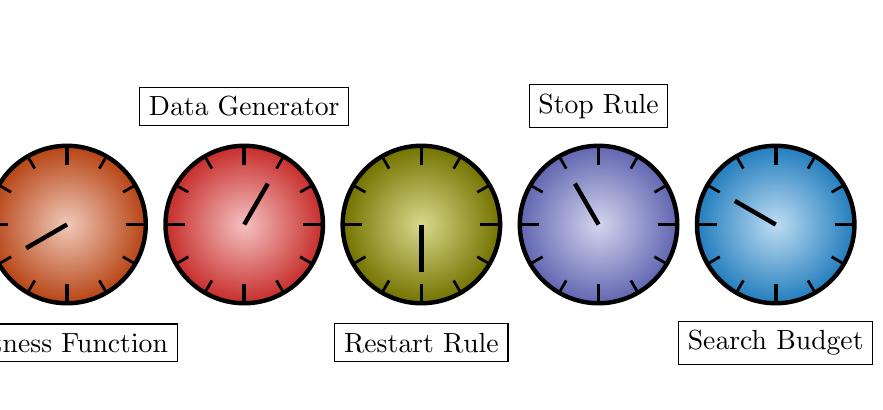
\begin{tikzpicture}[scale=1]

  \path[use as bounding box] (-0.5,2.5) rectangle (10,-2);

  \uncover<2->{
    \clock{0}{0}{clock0}{8};
    \node[draw] at (0cm,-1.5cm) {Fitness Function};
  }
  \uncover<3->{
    \clock{1}{0}{clock3}{1};
    \node[draw] at (2.25cm,+1.5cm) {Data Generator};
  }
  \uncover<4->{
    \clock{2}{0}{clock6}{6};
    \node[draw] at (4.50cm,-1.5cm) {Restart Rule};
  }
  \uncover<5->{
    \clock{3}{0}{clock9}{11};
    \node[draw] at (6.75cm,+1.5cm) {Stop Rule};
  }
  \uncover<6->{
    \clock{4}{0}{clock11}{10};
    \node[draw] at (9cm,-1.5cm) {Search Budget};
  }

\end{tikzpicture}

\hspace*{.33in}
\begin{tikzpicture}
  \path[use as bounding box] (-4.5,1) rectangle (10,-2);
  \path[->]<7-> node[special, text width=40ex]
    (Requirements) at (0,-.6)
    {{\Large How do parameter values \\ influence the efficiency of SBST?}};

\end{tikzpicture}

\end{overprint}
